\documentclass[12pt,openany,onecolumn]{book}
\usepackage{graphicx}
\usepackage{caption}
\usepackage{subcaption}
\usepackage{color}
\usepackage[table]{xcolor}
\pagestyle{plain}
\usepackage{hyperref}
\usepackage{fancyhdr}
\usepackage[headings]{fullpage}
\pagestyle{fancy}
\lhead{{\small ASAP FP7 Project}}
\rhead{{\small \delivtitle}}
\usepackage{times}
%\usepackage{helvet}
%\renewcommand{\familydefault}{\sfdefault}
\usepackage{amssymb,amsthm,amsmath,amsfonts}
\usepackage{lmodern}
\usepackage{textcomp}
\usepackage[T1]{fontenc}
\usepackage{multirow}
\usepackage{xspace}
\usepackage{pgfgantt}
\usepackage{pdflscape}
\definecolor{rowcolor}{rgb}{0.8,0.9,1}

\newtheorem{lemma}{Lemma}

\newcolumntype{P}[1]{>{\centering\arraybackslash}p{#1}}

\usepackage{mathtools} % Bonus
\DeclarePairedDelimiter\norm\lVert\rVert

\usepackage[acronym,nonumberlist,toc]{glossaries}
\usepackage{glossary-superragged}
% \newglossarystyle{modsuper}{%
%   \glossarystyle{super}%
%   \renewcommand{\glsgroupskip}{}
% }
\makeglossaries

\renewcommand*{\acronymname}{List of Acronyms and Abbreviations}
\renewcommand*{\glspostdescription}{} % remove trailing dot
\renewcommand{\glsnamefont}[1]{\textbf{#1}}
\newacronym{dag}{DAG}{Directed Acyclic Graph}
\newacronym{dg}{DG}{Directed Graph}
\newacronym{gui}{GUI}{Grafical User Interface}
\newacronym{wms}{WMS}{Workflow Management System}
\newacronym{wmt}{WMT}{Workflow Management Tool}
\newacronym{ipo}{IPO}{Input Processor Output}
\newacronym{es}{ES}{Exhaustive Search}
% \newacronym{bsp}{BSP}{Bulk Synchronous Parallel}
% \newacronym{hdfs}{HDFS}{Hadoop File System}

\newtheorem{definition}{Definition}
\newtheorem{proposition}{Proposition}
\newtheorem{theorem}{Theorem}
\newtheorem{example}{Example}

\usepackage{listings}
\renewcommand{\lstlistingname}{Algorithm}% Listing -> Algorithm
\lstset{
	backgroundcolor=\color{white},
	basicstyle=\footnotesize,
	breaklines=true,
	commentstyle=\color{lightgray},
	frame=single,
	numbers=left,
	numbersep=8pt,
	stepnumber=1,
	tabsize=2,
}

\def\delivtitle{Workflow Management Tool\\ {\small ASAP, {\rm \it technical report}}}

\begin{document}

\title{\delivtitle}
\author{}
\date{}
\newcommand{\eat}[1]{}

\thispagestyle{empty}
\begin{center}
\large
\textbf{FP7 Project ASAP} \\
Adaptable Scalable Analytics Platform\\[2\baselineskip]


\includegraphics[width=4cm]{asap-logo.png}\\[3\baselineskip]

{\Huge\bf \delivtitle}\\[3\baselineskip]
\end{center}

\textbf{Version History}
\begin{center}
\begin{tabular}{|l|p{3cm}|p{5cm}|p{3cm}|}
\rowcolor{gray}
\hline
Version & Date        & Author        & Comments \\
\hline
1.0 &  18 Aug 2015 & V. Kantere, M. Filatov & First Version \\
2.0	& 22  Aug 2015 & V. Kantere, M. Filatov & Final Version \\
\hline
\end{tabular}
\end{center}

\paragraph{Acknowledgement}
This project has received funding from the European Union's 7th Framework Programme for research, technological development and demonstration under grant agreement number 619706.

\paragraph{Abstract}
This work is a technical report on the first version of the Workflow Management Tool (WMT). This version incorporates the prototypes of three core modules of the WMT architecture, namely the Workflow Design, Analysis and Optimization modules. The report first gives a quick overview of the WMT architecture and then delves into the implementation details of each involved module.

\smallskip
\paragraph{Keywords} Workflow model, analysis, optimization, design tool.


\tableofcontents

\newpage
\phantomsection
\addcontentsline{toc}{chapter}{\listfigurename}
\listoffigures
\begingroup
\renewcommand{\cleardoublepage}{}
\renewcommand{\clearpage}{}
\phantomsection
\addcontentsline{toc}{chapter}{\listtablename}
\listoftables
\endgroup
% \printglossary[type=\acronymtype,title={List of Abbreviations}]
% \newpage


\chapter{Introduction}

\section{Workflow management tool overview}
The Workflow Management Tool (WMT) is a component of the ASAP system architecture. It is used for workflow creation, modification, analysis and optimisation.

WMT provides a GUI for workflow design. The model underlying WMT combines simplicity of expression of application logic and adaptation of the level of description of execution semantics. It enables the separation of task dependencies from task functionality. In this way, WMT can be easily, i.e. intuitively and in a straightforward manner, used by many types of users, with various levels of data management expertise and interest in the implementation.

The workflow and the including tasks are described using a JSON-based metadata language. The workflow is analysed and the result of the analysis can be a list of detected errors of a workflow or an analysed workflow which is actually an enhancement of the initial workflow with more vertices, substitution of vertices and/or edges in the initial workflow with others, and addition of metadata to the tasks.

WMT is a fully open-source\footnote{\url{https://github.com/maxfil/wmt}  - this will be changed to the ASAP repository} instrument that includes the designing interface, as well as analysis and optimisation modules.

\section{Purpose of the document}
This document serves as a report on the first version of the WMT and accompanies its prototype implementation. Its purpose is to delve into the implementation details of the core architectural modules. This includes the declaration semantics of the workflow, analysis and optimization techniques. Furthermore, we demonstrate the work of WMT on specific use-cases from D8.2 \cite{d8.2} and D9.2 \cite{d9.2}. Finally, we make an initial discussion on multi-workflow optimisation.

\section{Document structure}
The rest of this document is structured as follows:
\begin{itemize}
\item Chapter \ref{chapt:theory} gives a brief overview of the workflow model, including manipulation as described in D5.1 \cite{d5.1}. Moreover, it gives details on the workflow analysis and the workflow optimisation.
\item Chapter \ref{chapt:architect} presents details of the current architecture and implementation of WMT modules.
\item Chapter \ref{chapt:functionality} guides the reader on how to use the tool from creation up to optimisation, describing the functionalities and then gives examples of workflows driven by the use-case scenarios of D8.2 \cite{d8.2} and D9.2 \cite{d9.2}.
\item Chapter \ref{chapt:future} gives details on the current status of the formulation of some other optimisation objectives and multi-workflow optimisation and outlines our next steps.
\item Chapter \ref{chapt:related} summarises related work in the topic of the workflow optimization.
\item Chapter \ref{chapt:summary} concludes the technical report.
\end{itemize}

\chapter{Workflow management}\label{chapt:theory}
This chapter gives an overview of the workflow model, its analysis and its optimisation, as it is defined in D5.1 \cite{d5.1}, and gives details on what it is currently implemented in WMT. Moreover, it gives an update on our work in workflow optimisation.

\section{Workflow model}\label{sec:model}
The workflow represents applications as a directed acyclic graph (DAG) $G = (V, E)$. The vertices $V$ in the graph represent application logic and the edges represent the flow of data.
Application logic includes (a) the analysis of data, and (b) the modification of data. The edges $E$ are directed and connect the vertices that produce and consume data.
Each vertex in a workflow represents one or more tasks of data processing. Each task $T$ is a set of \emph{inputs}, \emph{outputs} and a \emph{processor}. In this text we also use the term \emph{operator} instead of the term \emph{processor}.
Tasks may share or not inputs, but they do not share processors and outputs. The inputs and outputs of the tasks of a vertex can be related to incoming and outgoing edges of this vertex, but they do not identify with edges: inputs and outputs represent consumption and production of data, respectively, and edges represent flow of data.

\begin{definition}
In a digraph $G$, the out-degree $d_G^{+}(v)$ is the number of edges leaving a vertex $v$, and the in-degree $d_G^{-}(v)$ is the number of edges entering a vertex $v$.
\end{definition}

\begin{definition}
A root is a vertex $v$ with in-degree $d_G^{-}(v) = 0$; and a sink is a vertex with out-degree $d_G^{+}(v) = 0$.
\end{definition}

A workflow has one root and several sink vertices. Data and operators can be either abstract or materialized. Abstract are the operators and datasets that are described partially or at a high level by the user when composing her workflow whereas materialized are the actual operator implementations and existing datasets, either provided by the user or residing in a repository. A generic tree-metadata format depicted as a subtree with a root \emph{`operator'} is shown in Figure \ref{fig:wtree}.
In Section 3.1.1 (Tree-metadata framework) of the report D3.2 \cite{d3.2} meta-data of data and operators are described in more detail.

\subsection{Workflow representation}\label{sec:format}
In WMT a workflow is represented in a single JSON file. 
This representation captures structural information, design metadata (e.g., functional and non-functional requirements, physical characteristics like resource allocation), operator properties (e.g., type, schemata, statistics, engine and implementation details, physical characteristics like memory budget), and so on.

\begin{figure}[h]
\centering
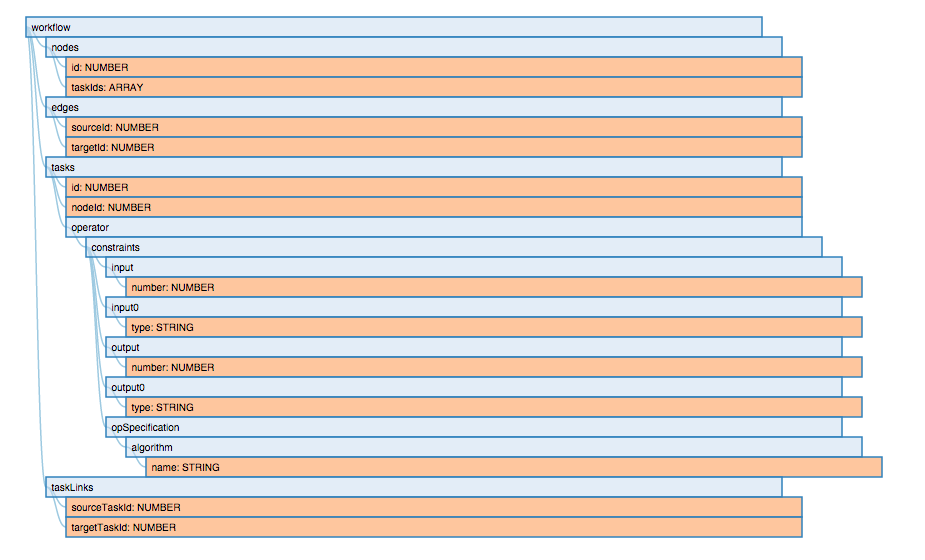
\includegraphics[width=\linewidth]{figs/wtree}
\caption{Workflow metada tree}\label{fig:wtree}
\end{figure}

The first levels of the metadata tree of the workflow are the following (shown in Figure \ref{fig:wtree}):
\begin{itemize}
\item \textbf{Nodes} Each node contains a list of task IDs which belong to this node.
\item \textbf{Edges} This is a list of pairs of node IDs - $(sourceId, targetId)$. An edge defines the flow of data from one vertex to another. These nodes are called the source and the target, respectively.
\item \textbf{Tasks} This part contains a list of task meta-data. The task meta-data consists of the information that is used to match abstract and materialized operators and datasets and the ID of a node to which this task belongs.
\item \textbf{TaskLinks} (optional) This part contains links between tasks lying within a single node.
\end{itemize}

\section{Workflow analysis}\label{sec:analysis}
The workflow structure alleviates from the user the burden of determining any or some execution semantics for the application logic. The execution semantics of the workflow includes the execution of tasks in vertices and the execution of input-output dependencies of edges. The determination of the execution semantics of vertices and edges leads to an execution plan of the workflow. We refer to this plan as the \emph{analysed} workflow. The latter is actually an enhancement of the initial workflow with more vertices, and substitution of vertices and/or edges in the initial workflow with others. 

More specifically, in the analysed workflow, an edge with different input and output metadata, may be replaced with two edges 
and a new vertex; the new vertex corresponds to a new task that takes the data and metadata of the input of the initial edge and produces the data and metadata of the output of the initial edge. In other words, since the data of the input and the output of an edge are equivalent, this task changes only the metadata. Such vertices are \emph{associative}, as they encompass associative tasks.
Also, a vertex that includes multiple tasks, in the original workflow, is replaced, in the analysed workflow, with a set of new vertices that each includes one task of the original vertex. The new vertices may or may not be connected with new edges.

Furthermore, in the analysed workflow, a vertex that corresponds to multiple tasks is replaced with an \emph{associative subgraph} that contains a set of new vertices that correspond to these tasks. This set contains vertices that correspond to the tasks of the initial vertex: each new vertex corresponds to one task; vertices may correspond 1-1 to tasks, but it can be the case that two or more vertices correspond to the same task\footnote{Replication of tasks using many associative vertices that correspond to the same task of an original vertex may be necessary for the optimisation of the workflow execution.}. Naturally, the incoming edges of the initial vertex may have to be replicated, since they may correspond to the input of more than one tasks. The outgoing edges, however, remain the same, as each corresponds to the output of one task. The replacing subgraph may also contain new edges that connect the replacing vertices. Such edges represent the dependencies between tasks related to their execution semantics, and not related to the semantics of the application logic, as expressed by the user.

\section{Workflow optimisation}\label{sec:optimisation}
In D5.1 \cite{d5.1} we have proposed two axes of a workflow optimization, namely: optimisation via graph reconfiguration and via optimal resource management. Currently, we focus on the first axis of optimisation, i.e. via the reconfiguration of the graph of the analysed workflow. To do this we employ methods for the manipulation of the workflow. A brief overview of these methods is provided below.

\subsection{Workflow manipulation}\label{subsec:transitions}
A workflow is manipulated so that it can be executed more efficiently than originally designed. Manipulation is performed using the following operations:

\begin{itemize}
\item \textbf{Swap.} The \emph{swap} operation applies to a pair of vertices, $v1$ and $v2$, which occur in adjacent position in an workflow graph $G$, and produces a new workflow graph $G'$ in which the positions of $v1$ and $v2$ have been interchanged. The goal of the \emph{swap} operation is to change the execution order of tasks. Currently, the WMT uses the \emph{swap} operation in the optimisation module.
\item \textbf{Merge.} The \emph{merge} operation takes as an input two vertices and produces one new vertex that includes the tasks of both initial vertices. The vertices that are merged can be connected with an edge, i.e. together they represent some task dependency(ies), or not, i.e. there is no task dependency between them. The goal of the \emph{merge} operation is to allow for a united optimisation of the tasks included in the two initial vertices, e.g. joint micro-optimisation on an execution engine. Currently, this operation is not yet implemented in the WMT.
\item \textbf{Split.} The \emph{split} operation takes as input one initial vertex and produces two new vertices that, together, include all the tasks included in the initial vertex. The two new vertices may or may not be connected. The goal of the \emph{split} operation is to lead to separate optimisation of subgroups of tasks included in the initial vertex. Currently, this operation is implemented in WMT and used to produce the \emph{analysed} workflow.
\end{itemize}

% Currently, we assume that we can \emph{swap} adjacent vertices for which their in-degree and out-degree equal to 1. Thus, the vertices order can be changed only within the line of sequential vertices without branching.

\subsection{Operator characteristics}\label{subsec:categories}
Workflow manipulation can be performed selectively depending on operator characteristics:

\begin{itemize}
\item \textbf{Blocking operators} require knowledge of the whole dataset, e.g., a grouping operator or an operator \emph{join} or \emph{sort}.
\item \textbf{Non-blocking operators} that process each tuple separately, e.g., operators \emph{filter} or \emph{calc}.
\item \textbf{Restrictive operators} output a smaller data volume than the incoming data volume, e.g. \emph{filter}.
\end{itemize}

Table \ref{table:categories} shows the operators that are currently in the operator library in WMT and their categorization.
\begin{table}[h]
	\centering
	\begin{tabular}{ |P{3cm}|P{2.5cm}|P{2.5cm}|P{2.5cm}| }
		\hline
		Operator & Blocking & Non-blocking & Restrictive \\
		\hline
		Filter &  & x & x \\
		\hline
		Calc &  & x & \\
		\hline
		Filter Join & x & & \\
		\hline
		groupBy Sort & x & & \\
		\hline
		PeakDetection & x & & \\
		\hline
		Tf-idf & x & & \\
		\hline
		k-Means & x & & \\
		\hline
	\end{tabular}
	\caption{Operator categorization}
	\label{table:categories}
\end{table}

The \emph{filter} operator returns all rows for which the <filter\_predicate> is `True'.
The \emph{calc} operator produces data with new attribute <calc\_attr> and value calculated by <calc\_expression>.
The others are obtained from the IRES platform.

For any operator that is added in WMT, the user has to define combinations of the new operator and operators already in the library, on which the \emph{swap} operation can be applied, if there are any such combinations. The WMT can use apply swapping on these predetermined combinations during the optimization stage. For example, the \emph{groupBy Sort}/\emph{filter} combination is swappable. However, the \emph{calc}/\emph{filter} combination is swappable or not depending on the specific implementation of \emph{calc}.

\subsection{Single-workflow optimization}\label{sec:singleworkopt}
We formulate the problem of optimizing a workflow for a single engine as a state space search problem. Starting with an initial workflow graph, we apply a set of graph transitions (see Section \ref{subsec:transitions}) to create new, equivalent graphs with (possibly) different costs. Applying transitions creates a large state space and the goal is to find an optimal workflow in this space with respect to the objective function (see Chapter \ref{chapt:future}).

We explore the state space exhaustively using the Exhaustive Search (ES). ES generates all possible states by applying all the applicable transitions to every state. The vastness of the state space requires more efficient exploration methods than the Exhaustive Search. To improve the search performance, a solution is to prune the state space. In the following, we propose techniques for achieving this.

Heuristics that can drive us close to the optimal solution quickly are the following:
\begin{itemize}
\item{\textbf H1:} Move restrictive operators to the root of the workflow to reduce the data volume, e.g., rather than \emph{extract \textrightarrow function \textrightarrow filter} do \emph{extract \textrightarrow filter \textrightarrow function}.
\item{\textbf H2:} Place non-blocking operators together and separately from blocking operators, e.g., rather than \emph{filter \textrightarrow sort \textrightarrow function \textrightarrow group} do \emph{filter \textrightarrow function \textrightarrow sort \textrightarrow group}.
\item{\textbf H3:} Parallelize non-blocking operators. Place adjacent operators on parallel paths, so that the latter can be executed on separate physical processors, e.g., if there are adjacent operators \emph{filter1 \textrightarrow filter2}, create two new paths in the workflow and  assign the \emph{filter1} and \emph{filter2} operators each to a different path, so that these workflow paths can run on separate processors concurrently. The workflow paths or, in general, parts, to be executed in parallel should be chosen such that their latency is approximately equal, i.e., if parallelization is possible on $n$ processors, break the flow into $n$ workflow parts $x_1, \ldots, x_n$ of equal (or near-equal) execution time, such that $max(time(x_i))$ is minimized.
\end{itemize}

Currently, the workflow optimization in WMT is carried out using the operation \emph{swap} and following the heuristics $H1$ and $H2$ (for the current form of the optimization algorithm see Section \ref{sec:optimizer}). 

\chapter{Workflow management tool architecture and implementation}\label{chapt:architect}

\begin{figure}[h]
\centering
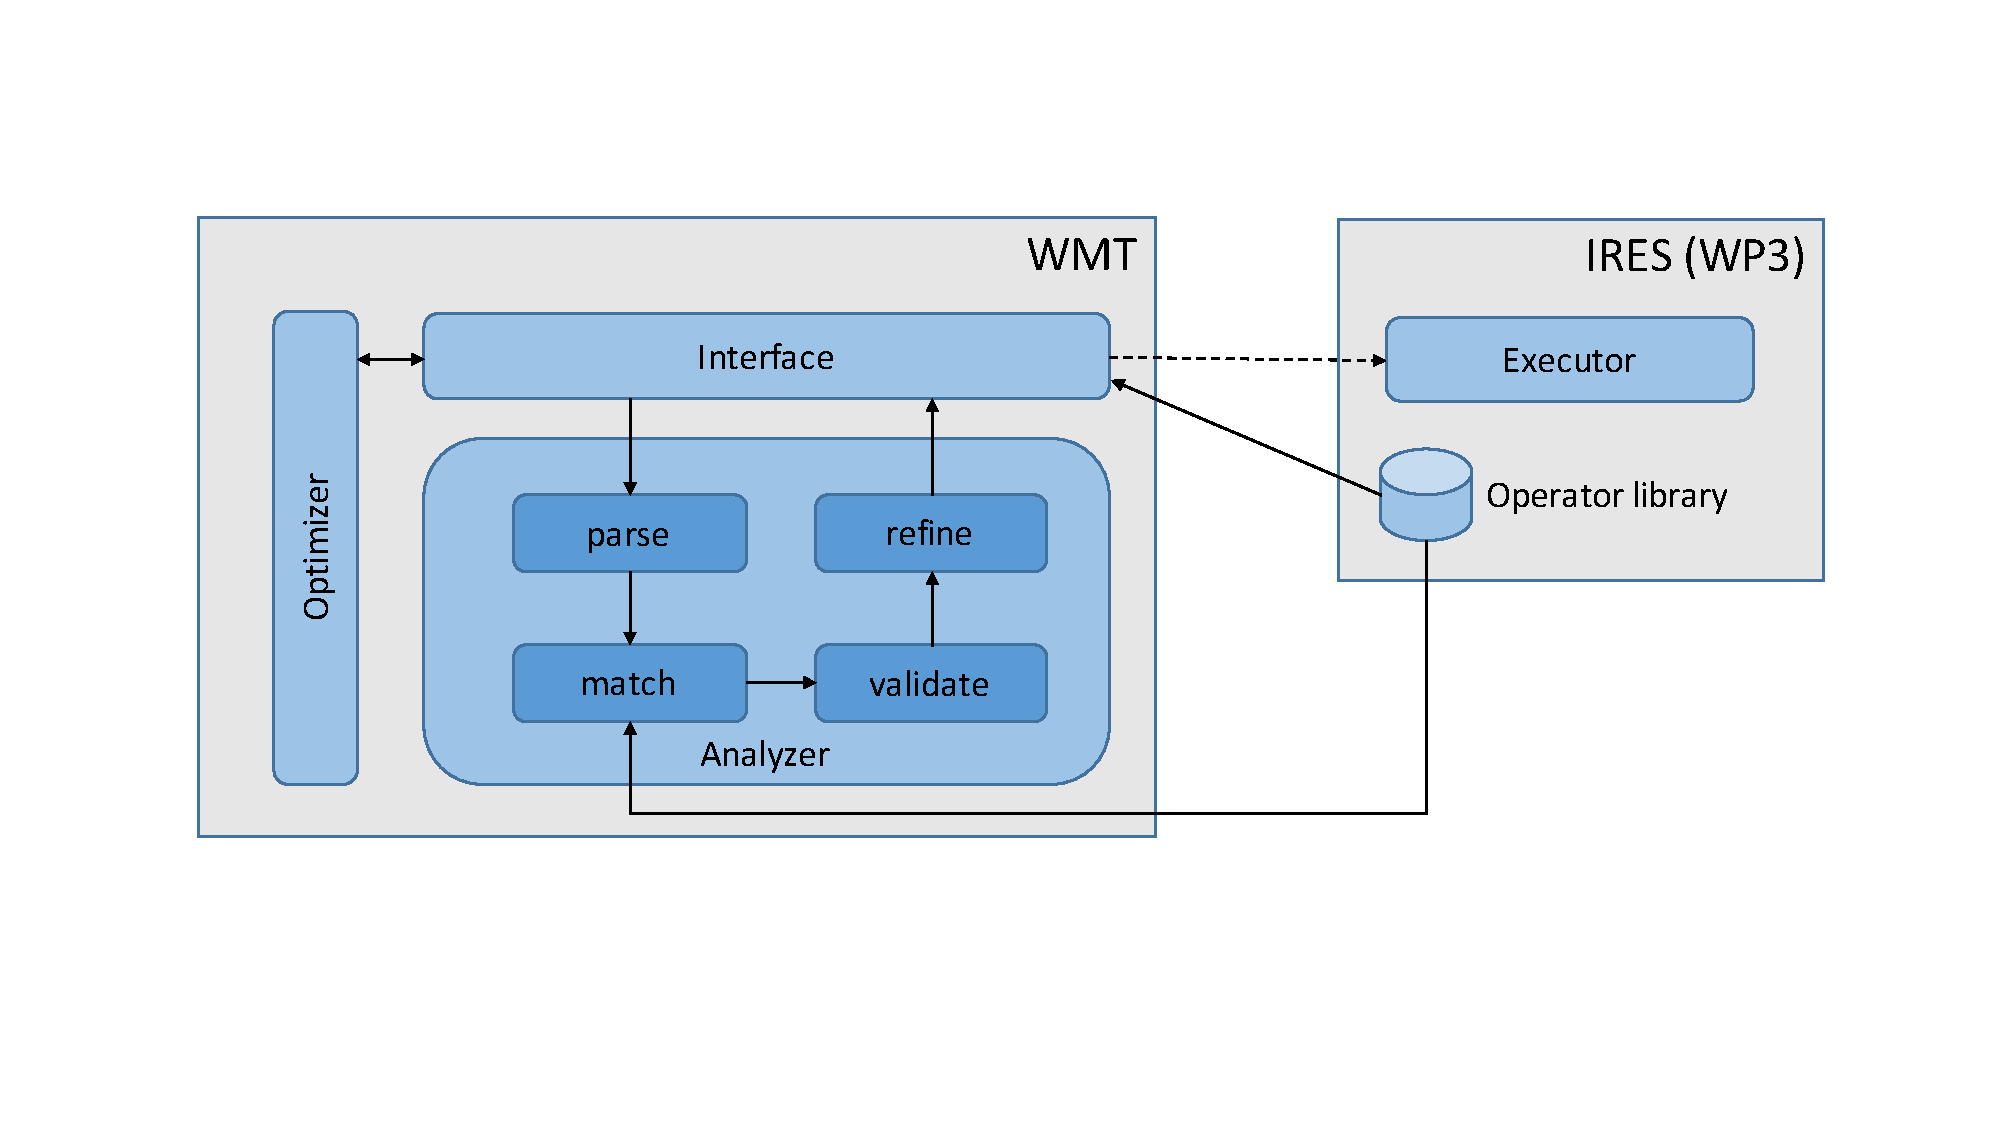
\includegraphics[width=\linewidth]{figs/architect}
\caption{The architecture of the WMT}\label{fig:architect}
\end{figure}

In this chapter, we describe in detail the current implementation of WMT. We discuss the architecture, the functionalities provided by the different modules and integration of WMT with other parts of ASAP. Figure \ref{fig:architect} depicts the architecture of WMT as well as its interaction with external components. The main components of the architecture are:
\begin{itemize}
\item \textbf{Interface.} The interface accepts a workflow definition in the representation described in Section \ref{sec:format}. It enables users to interactively create and/or modify a workflow.

\item \textbf{Analyzer.} The analyzer parses the workflow, identifies operators and data stores and maps them to a library of operators supported in WMT (See Section \ref{sec:integration}), generates metadata of edges, finds edges where the data conversion should be applied and adds the appropriate conversions.

\item \textbf{Optimizer.} The optimizer generates a functionally equivalent workflow graph optimized towards the performance objective (for more on the performance objective see Section \ref{sec:objectives}). 
\end{itemize}

These provide for workflow design, analysis and optimization. After their design, analysis and optimization, workflows are ready for their execution. They can be executed on independent engines and storage repositories, i.e. engines and repositories that may be accessed through other paths in ASAP (Section \ref{sec:integration}) or another third party platform, besides WMT.

\section{WMT architecture}\label{sec:interface}

\begin{figure}[h]
\centering
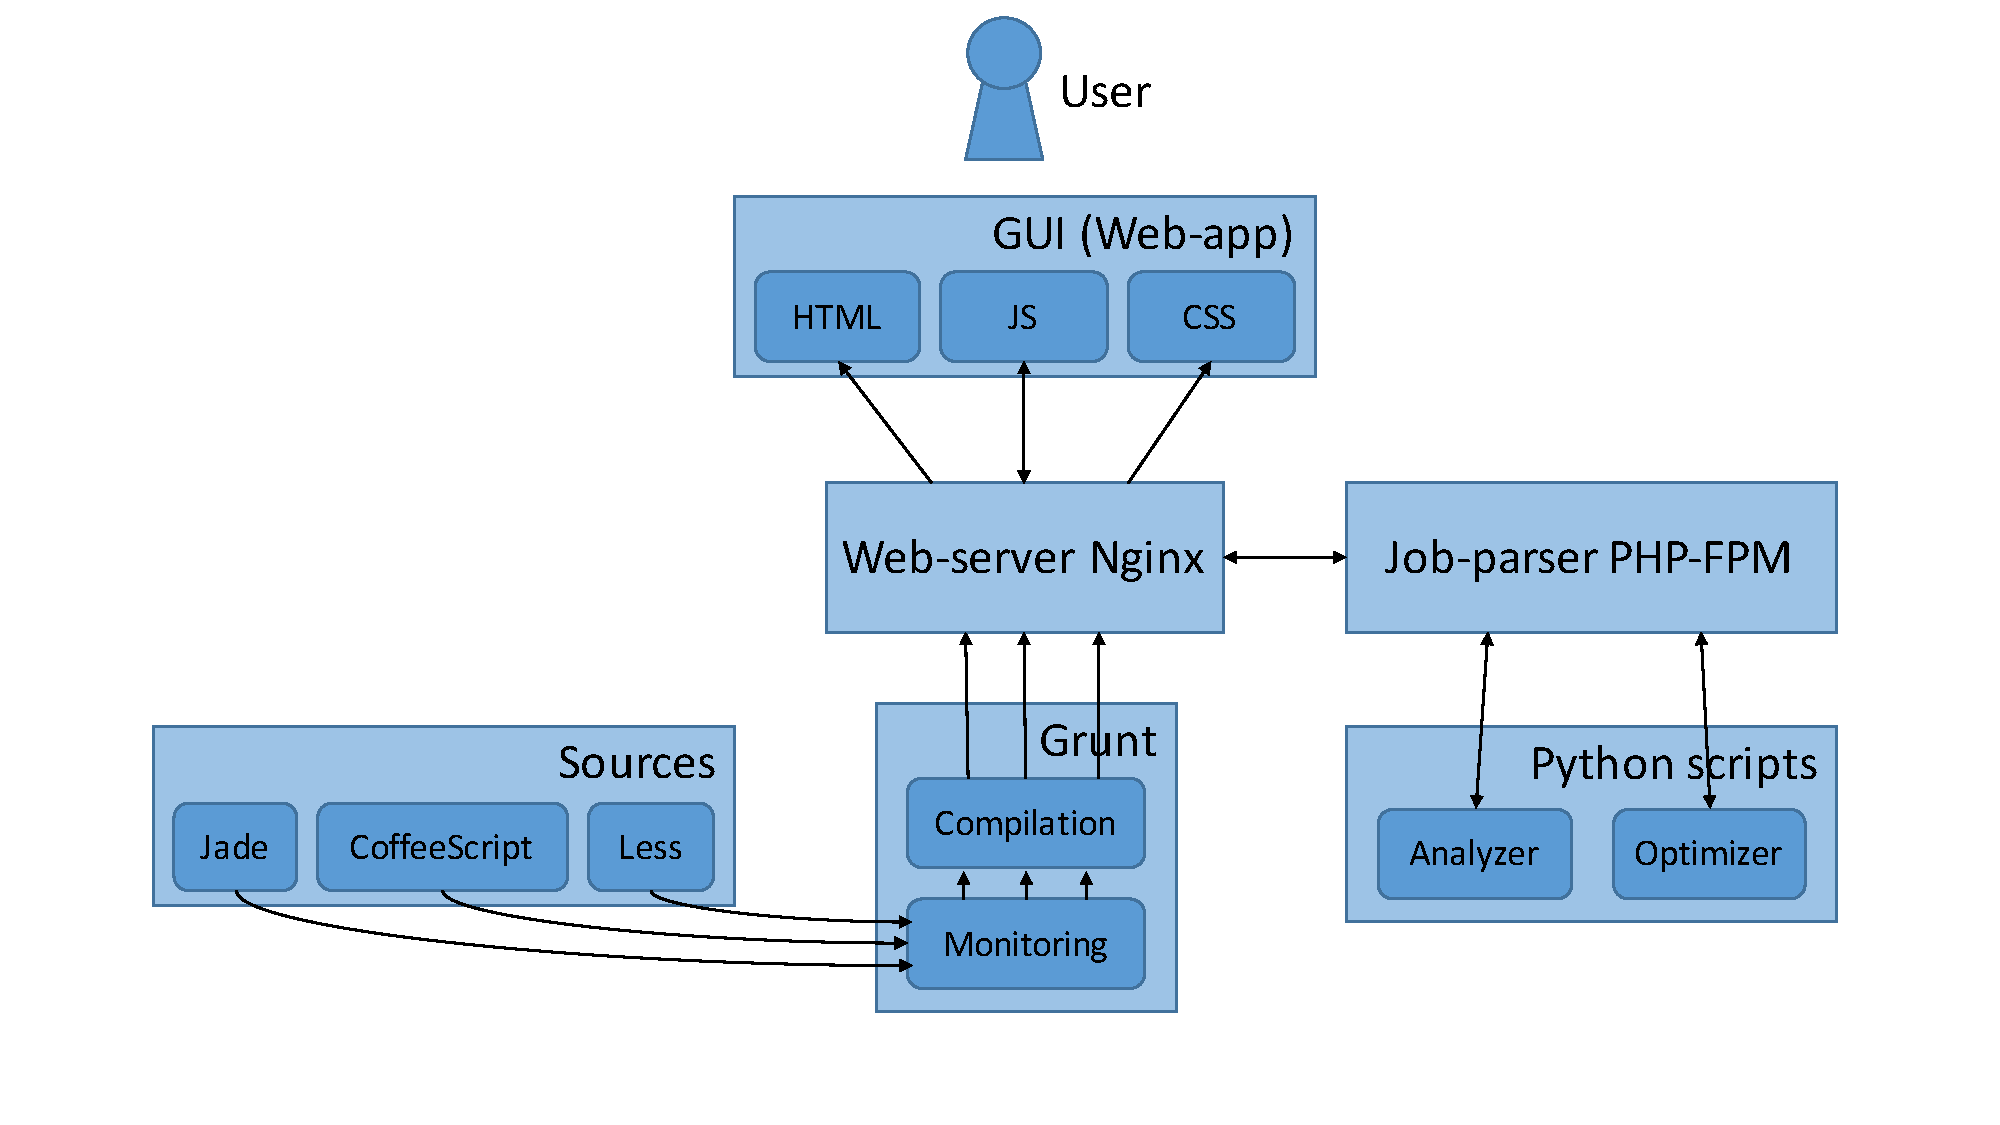
\includegraphics[width=\linewidth]{figs/tech_stack}
\caption{Technology stack used in WMT}\label{fig:tech_stack}
\end{figure}

WMT interface is a web application. It provides full functionality for designing a workflow even in the absence of server-side (Analyzer and Optimizer modules).
It is encoded in Hypertext Markup Language (HTML \cite{html}). To deliver content, WMT uses the Nginx \cite{nginx} web server. To encode business logic, WMT uses Javascript \cite{javascript} and PHP-FPM \cite{php-fpm}. The pages and scripts are compiled from Jade \cite{jade} and CoffeeScript \cite{coffescript} sources, respectively, using Grunt \cite{grunt}. The Analysis and Optimisation modules are scripts in Python \cite{python}. Figure \ref{fig:tech_stack} depicts the technical stack used in WMT and the interaction of WMT parts.


\section{Analyzer}\label{sec:analizer}
WMT analyses a workflow in several steps:
\begin{enumerate}
\item Parsing the workflow.
\item Categorizing operators (see Section \ref{subsec:categories}).
\item Validating consistency. A workflow is checked for the existence of cycles and correspondence of metadata of  adjacent nodes. Cycle discovery and metadata mismatch of adjacent nodes fall into the error list. The errors with the cycles cannot be resolved and the analysis stops and returns a list of errors back to the Interface. If possible, the data flow errors are solved by adding associative tasks in Step 6.
\item Generating metadata of edges. These are a joint result of input and output metadata of source and target nodes, respectively.
\item Splitting several tasks in a single node to several single-task nodes.
\item Augmenting the workflow with associative tasks. Currently, the implemented tasks are converting data flow: buffer and format conversion.
\end{enumerate}

\section{Optimizer}\label{sec:optimizer}
The Optimizer works on the analyzed workflow, where tasks have been categorized and each node has a single task.
Currently, the Optimizer uses heuristics $H1$ and $H2$ described in Section \ref{sec:singleworkopt}. These move restrictive operators towards the root of the workflow and place non-blocking operators together and separately from blocking operators.

The current form of the optimization algorithm follows all paths in a workflow by encountering all edges. It swaps nodes following the heuristics. It stops when no more swaps can be performed and an optimized version is produced (See Algorithm \ref{lst:optimisation}).

\begin{lstlisting}[caption={Optimization algorithm}, label={lst:optimisation}, language=Python, firstnumber=1, mathescape=true]
Input: An initial workflow $W$
Output: An optimized by two heuristics equivalent workflow state $W^o$
$W = (nodes, edges, tasks)$
while $swaps <> 0$ do
	$swaps = 0$
	for edge in edges do
		$source = nodes[edge[sourceId]]$
		$target = nodes[edge[targetId]]$
		if $d_G^{+}(source) <> 1$ or $d_G^{-}(source) <> 1$ then
			continue
		if $d_G^{+}(target) <> 1$ or $d_G^{-}(target) <> 1$ then
			continue
		# heuristic 1
		if $category(task(source))$ is $`restrictive'$ then
			continue
		if $category(task(target))$ is $`restrictive'$ then
			$swap(source, target)$
			$swaps++$
			continue
		# heuristic 2
		if $category(task(source))$ is $`non-blocking'$ then
			continue
		if $category(task(target))$ is $`non-blocking'$ then
			$swap(source, target)$
			$swaps++$
			continue
$W^o = (nodes, edges, tasks)$
return $W^o$ end
\end{lstlisting}

%On the next step of the integration
%In future
In the future, the Optimizer will be based on processing estimations of a workflow, which will be derived from IRES Executor and Profiler. Then, the heuristics will be used to prune the state space as it was described in Section \ref{sec:optimisation}.

\section{Integration}\label{sec:integration}

\begin{figure}[h]
\centering
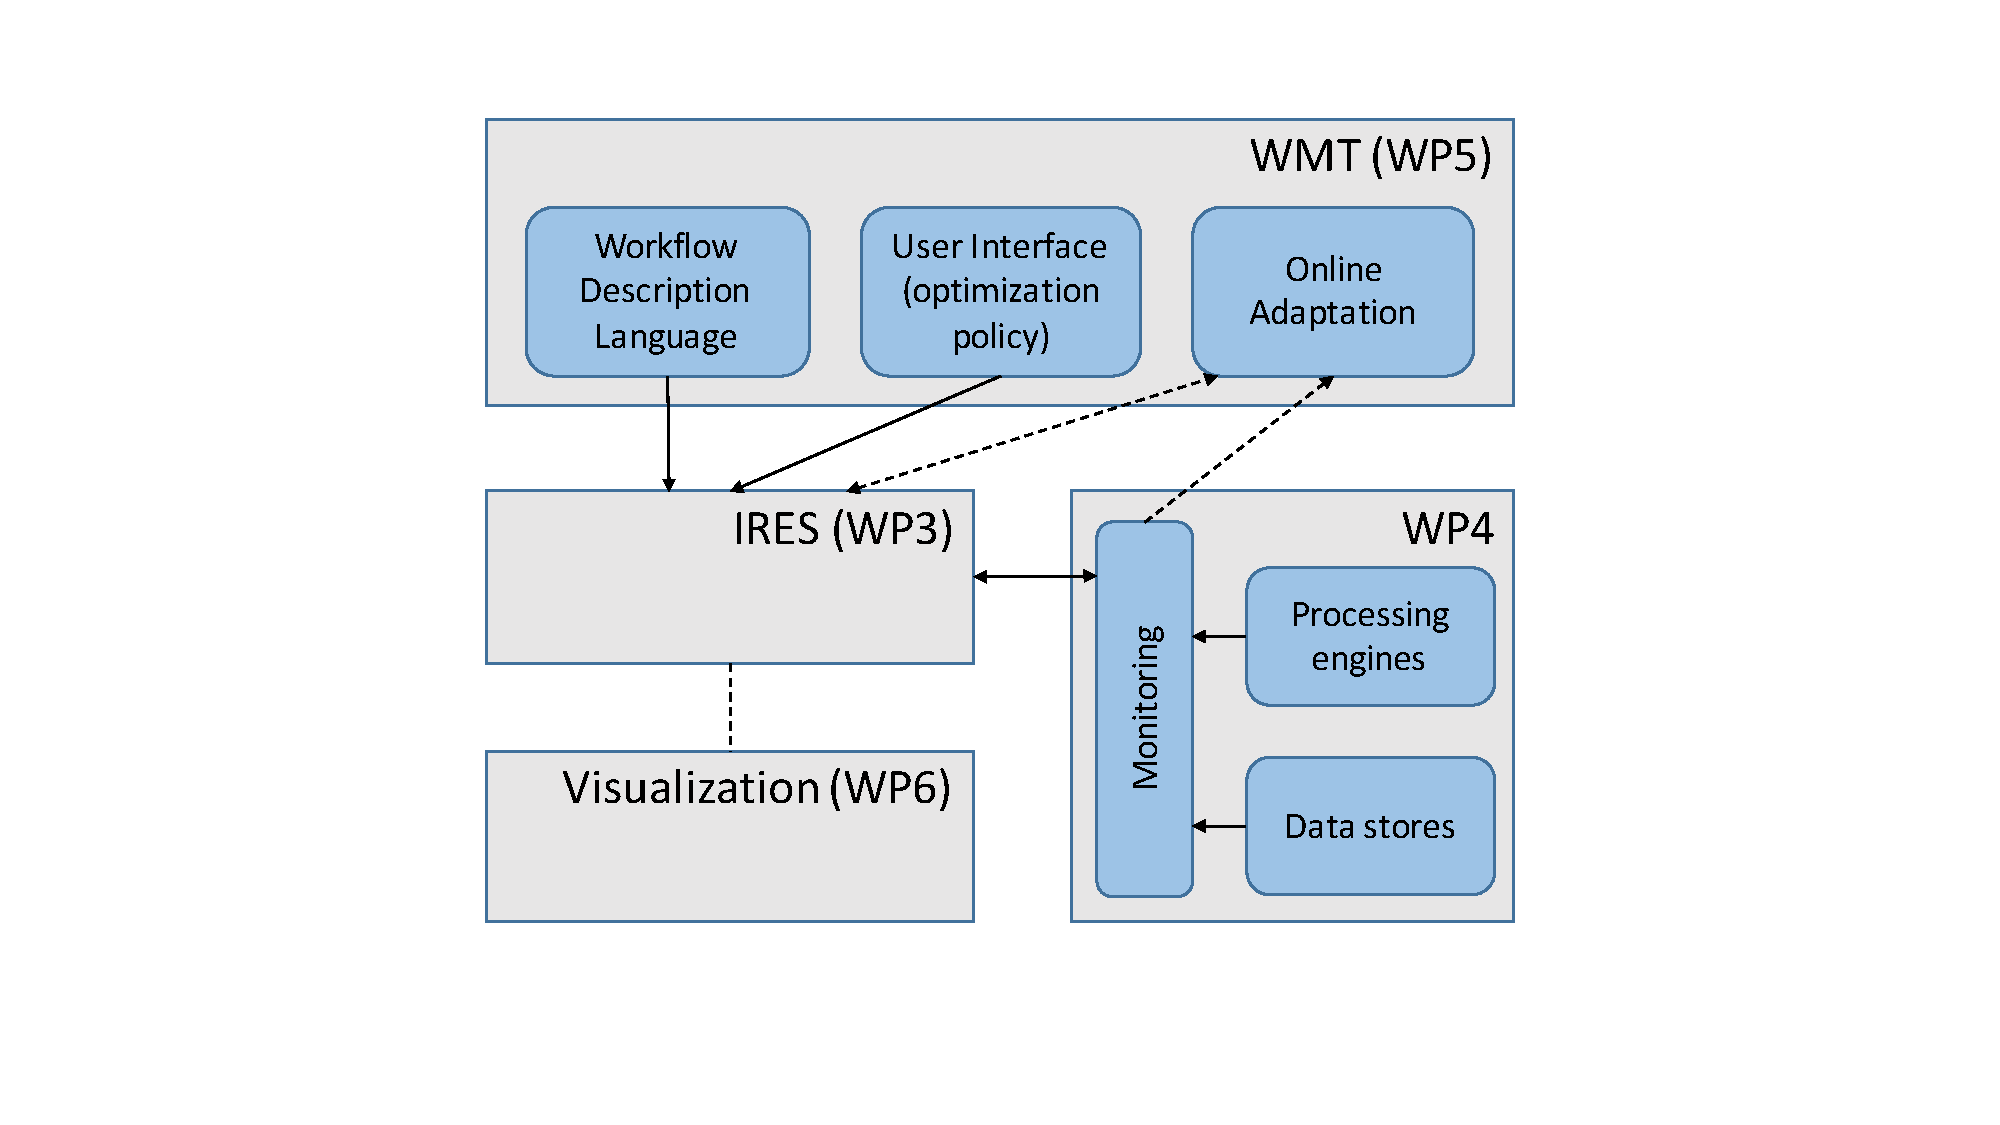
\includegraphics[width=\linewidth]{figs/ASAP_scheme}
\caption{WMT interaction with the rest components of ASAP}\label{fig:ASAP_scheme}
\end{figure}

IRES is a component of the ASAP that executes workflows (See D3.2 \cite{d3.2}), therefore WMT will have a tight integration with it (Figure \ref{fig:ASAP_scheme}). Currently WMT uses the Tree-metadata language (See 3.1.1 in the document D3.2 \cite{d3.2}) to express operators and receives a list of existing operators from IRES (See 2.3 in the document D3.2 \cite{d3.2}).

\chapter{Workflow management tool functionality}\label{chapt:functionality}

\section{GUI}\label{sec:gui}

\begin{figure}[h]
\centering
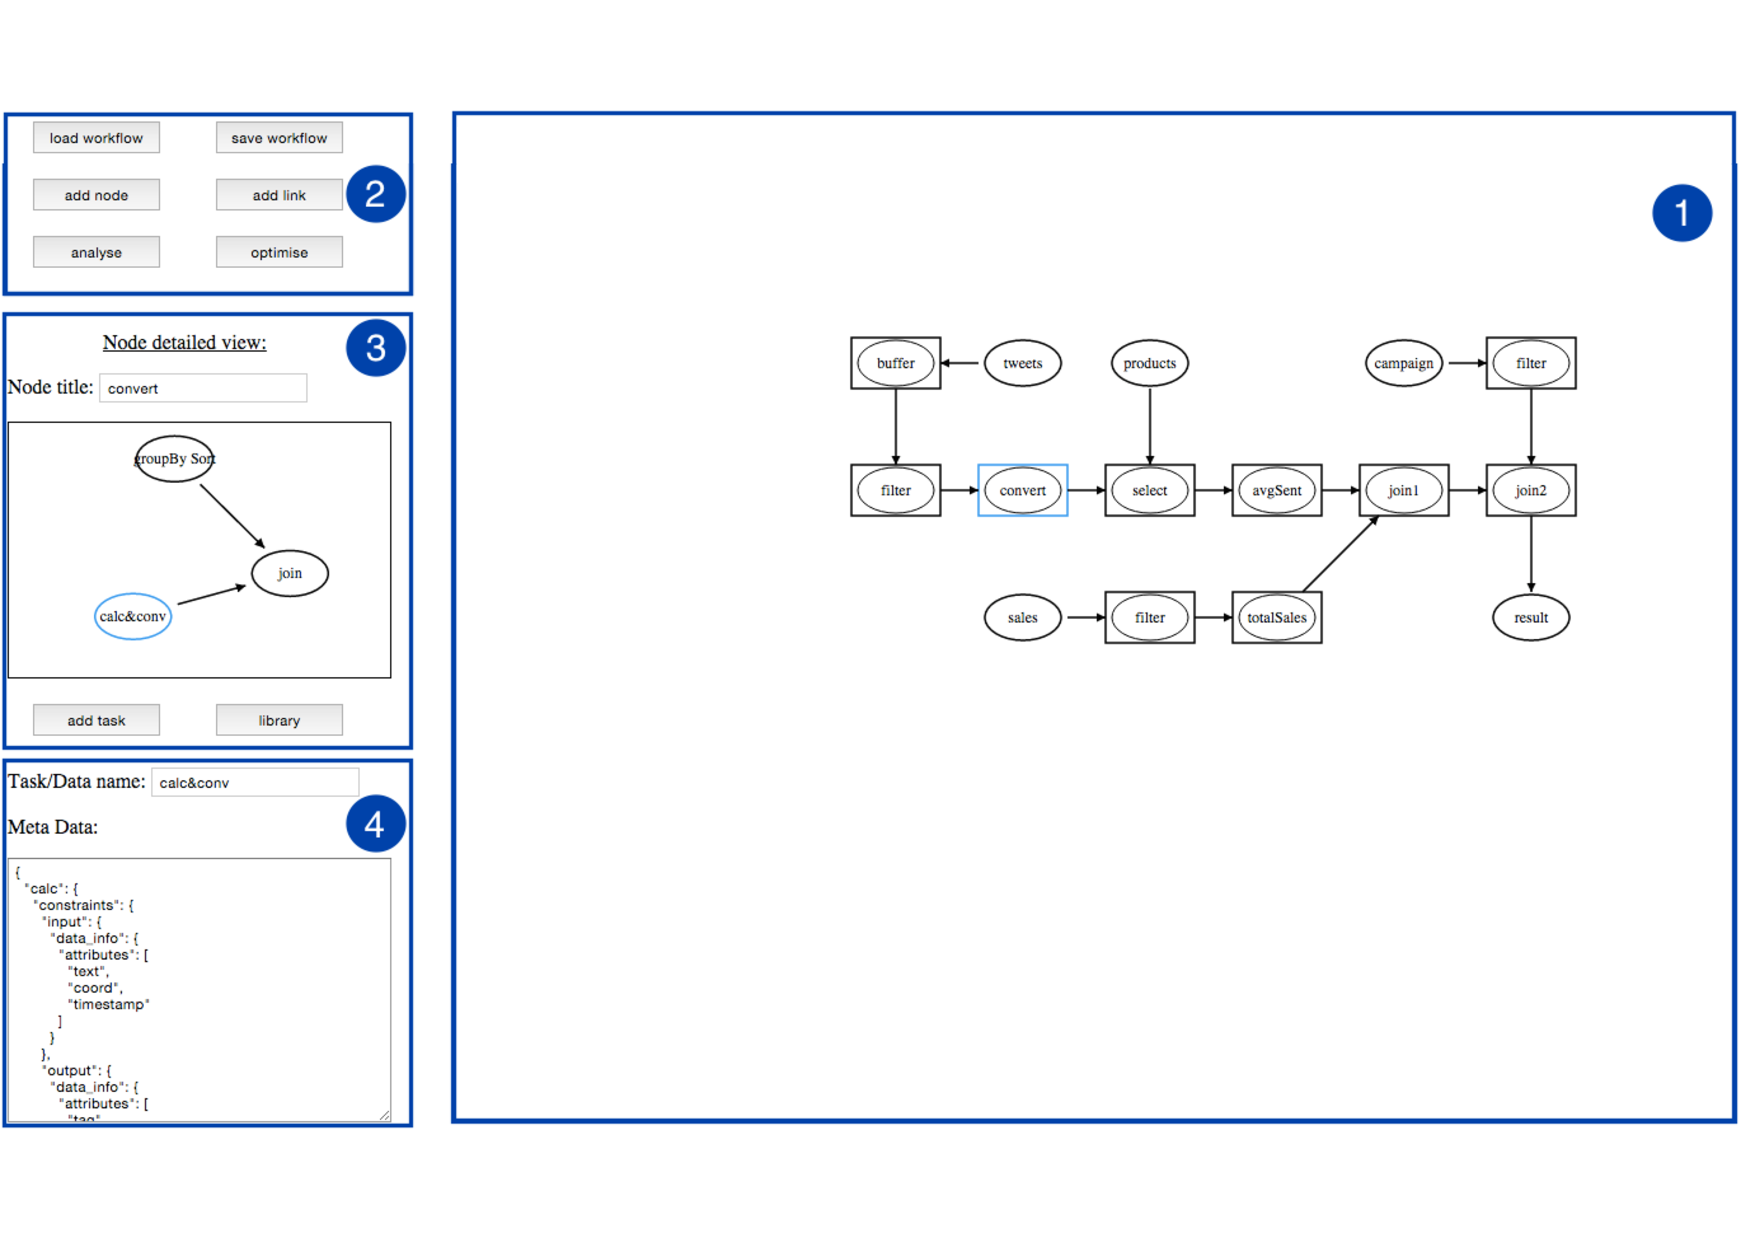
\includegraphics[width=\linewidth]{figs/scheme}
\caption{GUI of WMT}\label{fig:scheme}
\end{figure}

\begin{figure}[h]
\centering
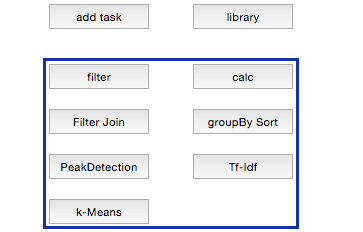
\includegraphics[scale=0.75]{figs/lib_buttons}
\caption{List of library operators}\label{fig:lib_buttons}
\end{figure}

WMT provides a GUI to enable users to design workflows and perform analysis and optimization.
The GUI consists of several areas (Figure \ref{fig:scheme}) that perform the following functions:
\begin{itemize}
\item Display the workflow (Area 1).
\item Add nodes and edges (Area 2). This process depicted in Figure \ref{fig:steps}. First, the user adds a node, then she adds two tasks in it from the operators library, and finally she connects nodes and tasks.
\item Create a new workflow from scratch, save and load it.
\item Perform workflow analysis or optimization.
\item Add tasks from a library (see Figure \ref{fig:lib_buttons}) or create new ones (Area 3). If the user adds a task from a library then it is accompanied by a set of metadata, i.e., properties that describe them. If a new task is created then the first levels of the metadata tree are predefined but users can add their ad-hoc subtrees to define their custom data or operators.
\item Display metadata of the selected task (Area 4).
\end{itemize}

\begin{figure}[h]
\centering
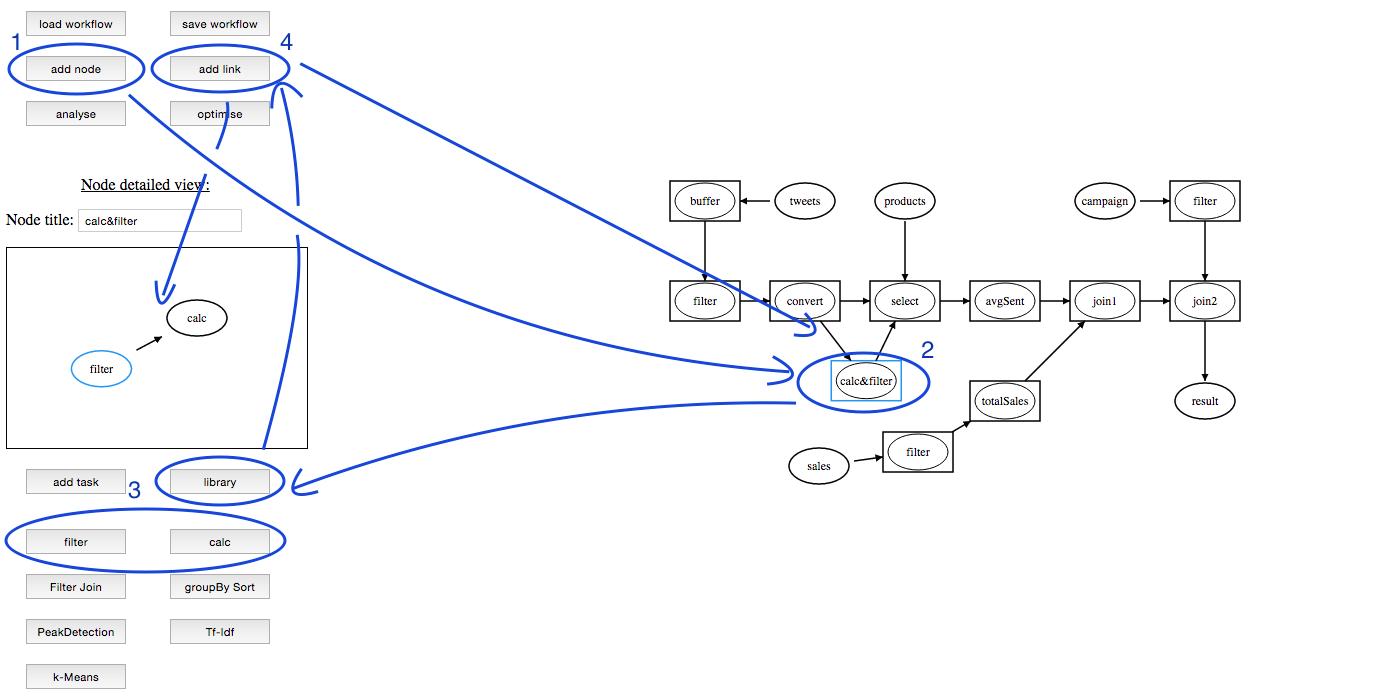
\includegraphics[width=\linewidth]{figs/steps.png}
\caption{Steps of adding node}\label{fig:steps}
\end{figure}

\section{Examples}\label{sec:examples}
The ASAP focuses on the real-time analysis of Web content and telecommunications data. This section presents several indicative use-cases selected based on their relevance to the ASAP research.

\subsection{Web content analytics}
The use case in this domain are centered on the services by Internet Memory Research as part of the Mignify platform (\url{www.mignify.com}). These services provide access to a very large collection of contents extracted from the Web, cleaned, annotated and indexed in a distributed infrastructure mainly based on Hadoop components. ASAP focuses on extending and enriching the public workflow interface supplied by Mignify, referred to as pipes (queries associated with a set of intelligent agents to extract or transform large-scale web data).

\subsubsection{Stream processing}
This use case captures a typical form of the current IMR Web analytics pipeline. Figure \ref{fig:use_case_nlp} presents a workflow for this use case. Data are selected from the document store based on some conditions (\emph{select}). These data are processed in order to extract some text (\emph{calc}), and the extracted text is moved to a different data store and stored there with other text and annotations (\emph{move}). The output data are further processed via NLP-classification.

\begin{figure}[h]
\centering
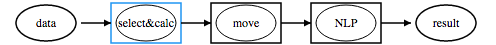
\includegraphics[width=\linewidth]{figs/nlp}
\caption{Workflow for NLP-classification}\label{fig:use_case_nlp}
\end{figure}

Figure \ref{fig:use_case_nlp_analysed} shows the result of the analysis module. The node containing two tasks select and calc has been split into two single-task nodes.

\begin{figure}[h]
\centering
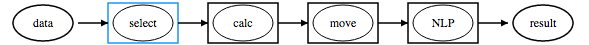
\includegraphics[width=\linewidth]{figs/nlp-a}
\caption{Workflow for NLP-classification}\label{fig:use_case_nlp_analysed}
\end{figure}

\subsection{Telecommunications data}
Call Detail Records (CDR) data is a good proxy to understand human mobility. The sheer volume of this data poses new challenges when extracting and visualizing specific indicators. ASAP investigates applications such as the following:

\subsubsection{Peak detection}
This use case involves processing of the anonymised CDR data of the past day by first selecting a spatial region and a temporal period (\emph{select}). For this region and period, the number of calls is calculated (\emph{calc}). Data and calculations from CDR are archived (\emph{archive}) in other storage (\emph{history}). After calls are counted, the application proceeds with algorithmic processing that detects peaks (\emph{calc2}). The objective of this processing is to detect peaks in load, according to a set of criteria. Criteria may include the minimum size of a region and/or period, the cut-off distance, or other parameters for selecting regions and periods. These parameters should be adjustable by the analytics engineer, marketing expert, etc., who uses the peak analysis results. The results of this workflow are added to a database (relational or graph DBMS) that contains peaks detected in previous data. The database of peaks can then be queried by a user to discover clusters of calls that occur with regularity e.g., every week, discover clusters of calls that occur without any regularity, or similar ad-hoc queries based on the pre-computed peak data. The workflow for this use case is shown in Figure \ref{fig:use_case_peaks}.

\begin{figure}[h]
\centering
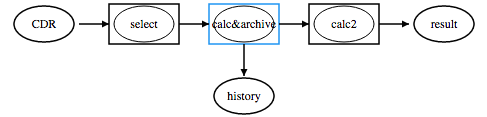
\includegraphics[scale=0.75]{figs/peakdetection}
\caption{Workflow for the detection of peaks}\label{fig:use_case_peaks}
\end{figure}

Figure \ref{fig:use_case_peaks_analysed} shows the result of the analysis module. The node containing two tasks calc and archive has been split into two single-task nodes.

\begin{figure}[h]
\centering
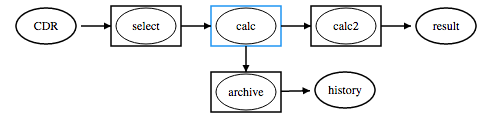
\includegraphics[scale=0.75]{figs/peakdetection-a}
\caption{Analysed workflow for the detection of peaks}\label{fig:use_case_peaks_analysed}
\end{figure}

\subsection{Marketing analytics}
Figure~\ref{fig:use_tweets} displays workflow of an analysis of a product marketing campaign. It combines sales data with sentiments about that product gleaned from tweets crawled from the Web. The result consists of total sales and average sentiment for each day of the campaign. Campaigns promote a specific product and are targeted at non-overlapping, geographical regions. To simplify the presentation, we assume the sentiment analysis of a tweet yields a single metric, i.e., like or dislike the product over a range of -5 to +5.

\begin{figure}
\centering
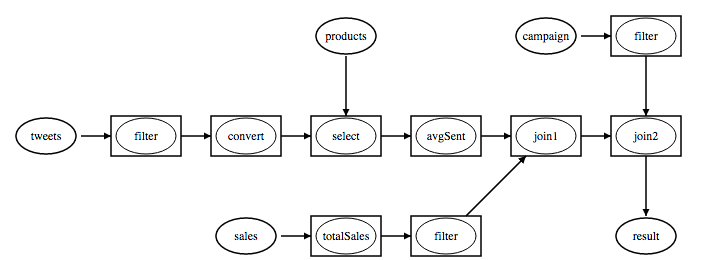
\includegraphics[width=\linewidth]{figs/tweets}
\caption{Workflow analysing a product marketing campaign}\label{fig:use_tweets}
\end{figure}

Figure~\ref{fig:use_tweets_analysed} represents an analysed workflow.
The Analyzer adds an associative tasks \emph{buffer}. It has been added to convert streaming data to batch.
\begin{figure}
\centering
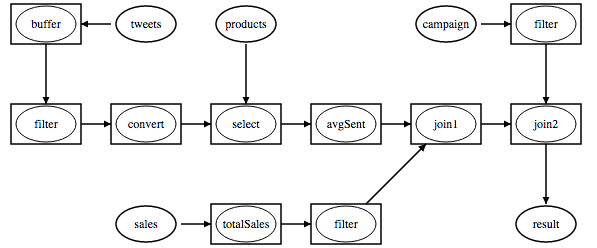
\includegraphics[width=\linewidth]{figs/tweets-a}
\caption{Analysed workflow for the marketing analytics}\label{fig:use_tweets_analysed}
\end{figure}

Figure~\ref{fig:use_tweets_optimised} depicts the result of the Optimizer work. It swapped vertices totalSales calculation and filtering of sales data.
\begin{figure}
\centering
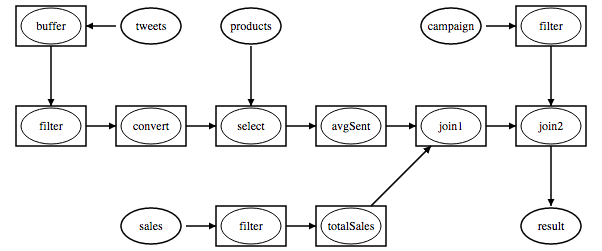
\includegraphics[width=\linewidth]{figs/tweets-o}
\caption{Optimised workflow for the marketing analytics}\label{fig:use_tweets_optimised}
\end{figure}

\chapter{Ongoing and future work}\label{chapt:future}

This chapter presents ideas that are towards a multi-workflow optimization.

\section{Performance objective}\label{sec:objectives}
\textbf{Performance} is a metric of workflow execution expressed in terms of time and used resources.

Let $W = \{W_1,\ldots W_n\}$ be a list of workflows. These workflows arrive at time points $T^a = \{t^a_1,\ldots t^a_n\}$. These two lists are not fixed, but changing over time as new workflows are added. The sizes of lists are equal and initially the list of times consist of zeros and $\forall i < j, t^a_i \leq t^a_j$. Workflow $W_{(n+1)}$ arrives at $t^a_{(n+1)}$ and these elements append to the lists and so on.

A workflow $W_i$ is a graph $G$ as defined by the workflow model. Each manipulation operation (see Section \ref{subsec:transitions}) transforms a workflow graph $G$ into an equivalent graph $G'$. In other words, if an operation $f$ is applied on a workflow $W_i$ it produces a new workflow $W'_i$: $W'_i = f(W_i)$. Two workflows are equivalent if they produce the same output, given the same input.

All possible equivalent workflows, or else, workflow states, can be produced by applying all the applicable operations to every equivalent workflow state. We denote as $SL(W_i) = \{W^1_i,\ldots W^k_i\}$  the list of all equivalent workflow states.
%
$T^s = \{t^s_1,\ldots t^s_n\}$ and $ T^e = \{t^e_1,\ldots t^e_n\}$ are the lists of start and end times of execution for workflows  respectively.

The goal is to minimize the total elapsed time of completion of the execution of workflows:
$$\min\limits \sum_{i=1}^{n} (t^e_i-t^a_i)$$
%As the workflows arrives continuously, the limit superior may not exist.
The end time of execution $t^e$ of a workflow depends on the starting time of execution $t^s$, as well as the \emph{processing cost} $C$ of this workflow. The cost $C$ is related to the time intervals the workflow is processed on one or several machines (i.e. a parallelized execution) and depends on the state of the system, (i.e. the utlization of resources by a pool of workflows), at a specific point in time. 
Consequently, the objective function is:
$$OF(t) = \min\sum_{i=1}^{n(t)} (t^s_i-t^a_i+C(W_i,t))$$

%As the processing cost $C(W_i,t)$ of a workflow depends on the state of the system (pool of workflows etc.). 
The estimations of the processing cost of workflows will be an input from the IRES platform.

\section{Multi-workflow optimization}
Beyond optimising single workflows, we will explore the optimisation of multiple workflows. We will aim to find common or similar subgraphs that we can optimise once and execute once or a few times. 

\begin{definition}{A `common part'}
\label{def:commonpart}
is a subgraph that is part of two or more workflows; these parts are bijective and corresponding operators in vertices are equivalent.
\end{definition}

Thus, our approach for multi-workflow optimization will be the joint execution of common parts (Definition \ref{def:commonpart}). We will try to rearrange workflows with common parts in order to enable such execution (see Figure \ref{fig:synccom}). 

\begin{figure}[h]
\centering
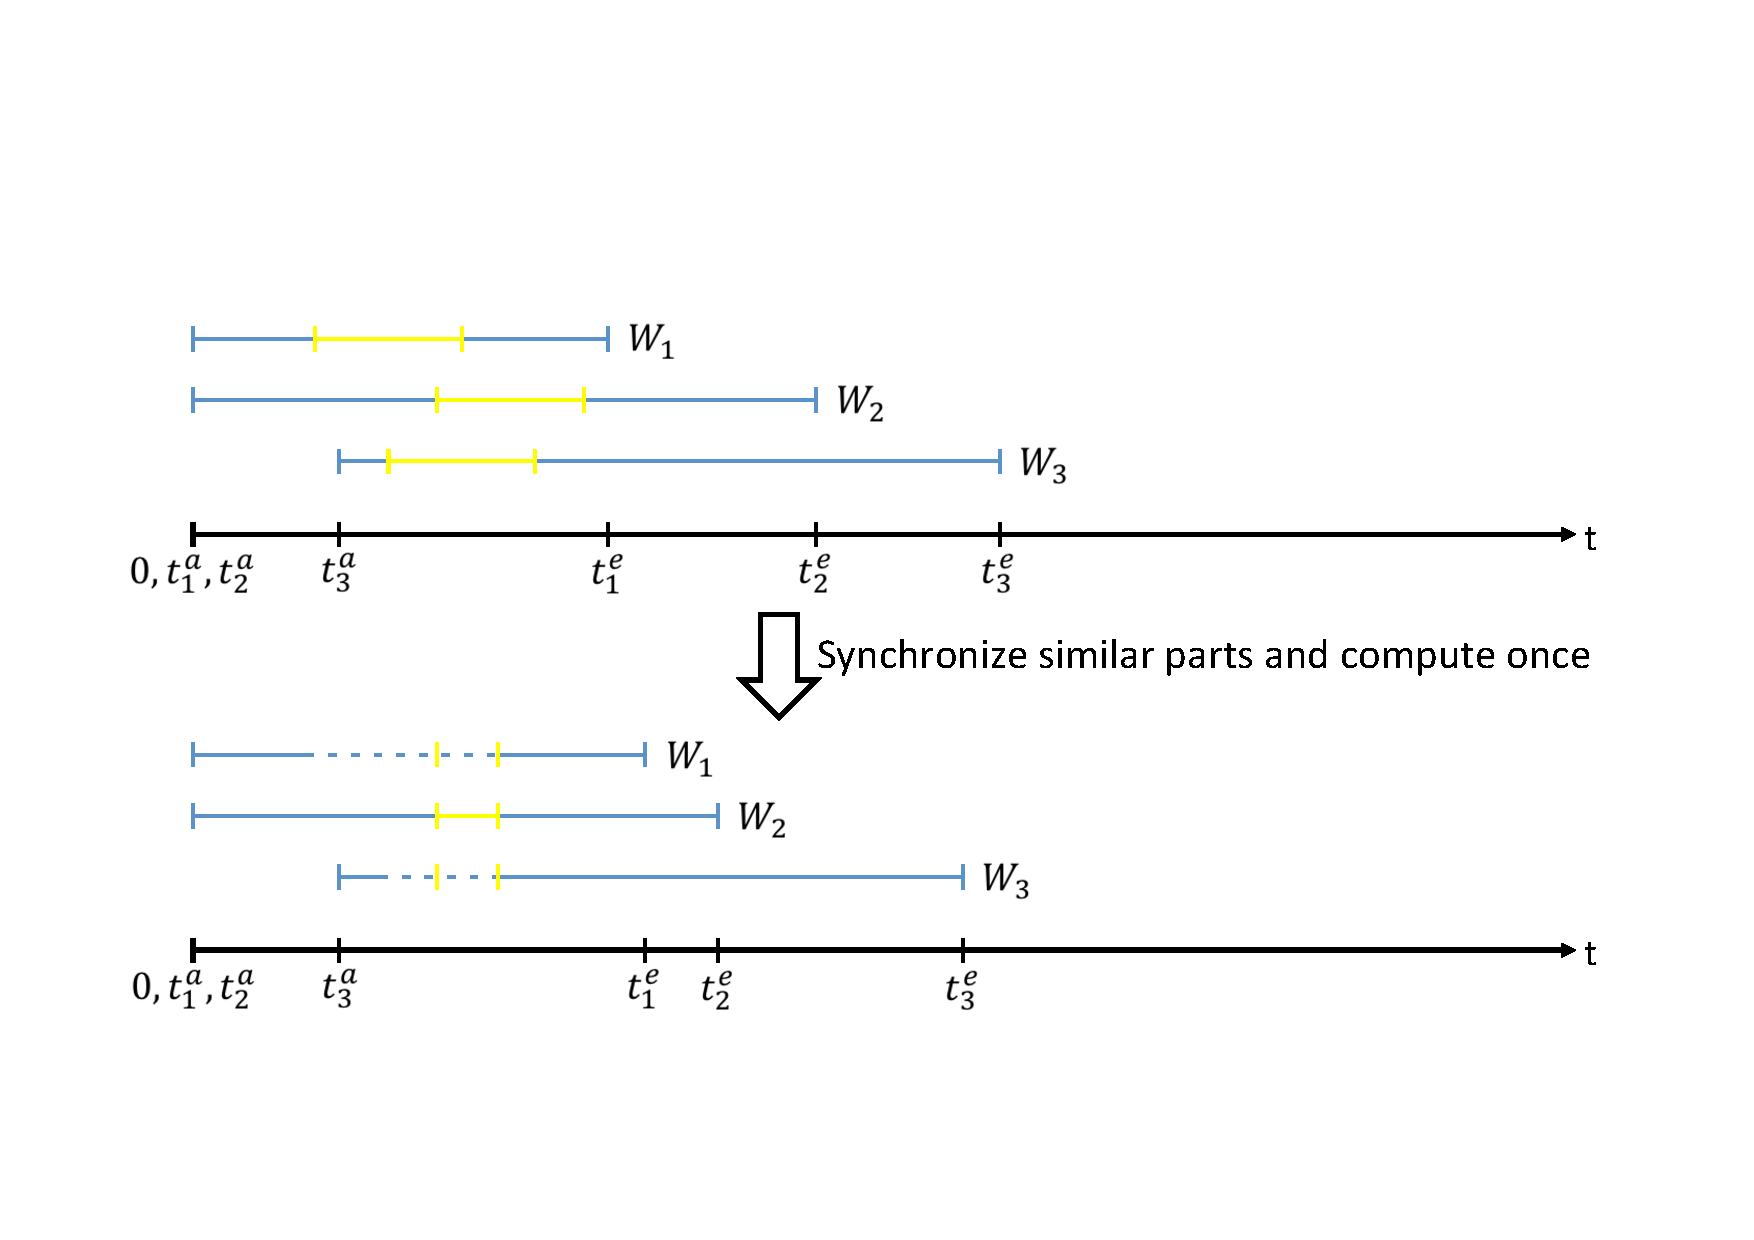
\includegraphics[width=0.6\linewidth]{figs/synccommonparts}
\caption{Synchronisation of common parts of multiple workflows}\label{fig:synccom}
\end{figure}

However, there are cases of workflows with common parts for which such rearrangement, and, therefore, joint execution of common parts, is not possible. Such cases occur if subgraphs of common parts have dependencies on subgraphs of other common parts. We introduce the terminology of `mutual arrangement' of subgraphs:
\begin{definition}
A vertex $v$ is reachable from another vertex $u$, if there is a directed path that starts from $u$ and ends at $v$.
\end{definition}

\begin{definition}
A subgraph $S$ depends from a vertex $v$, if there exists a vertex $u$ in the subgraph and $u$ reachable from $v$.
\end{definition}

\begin{figure}[h]
\centering
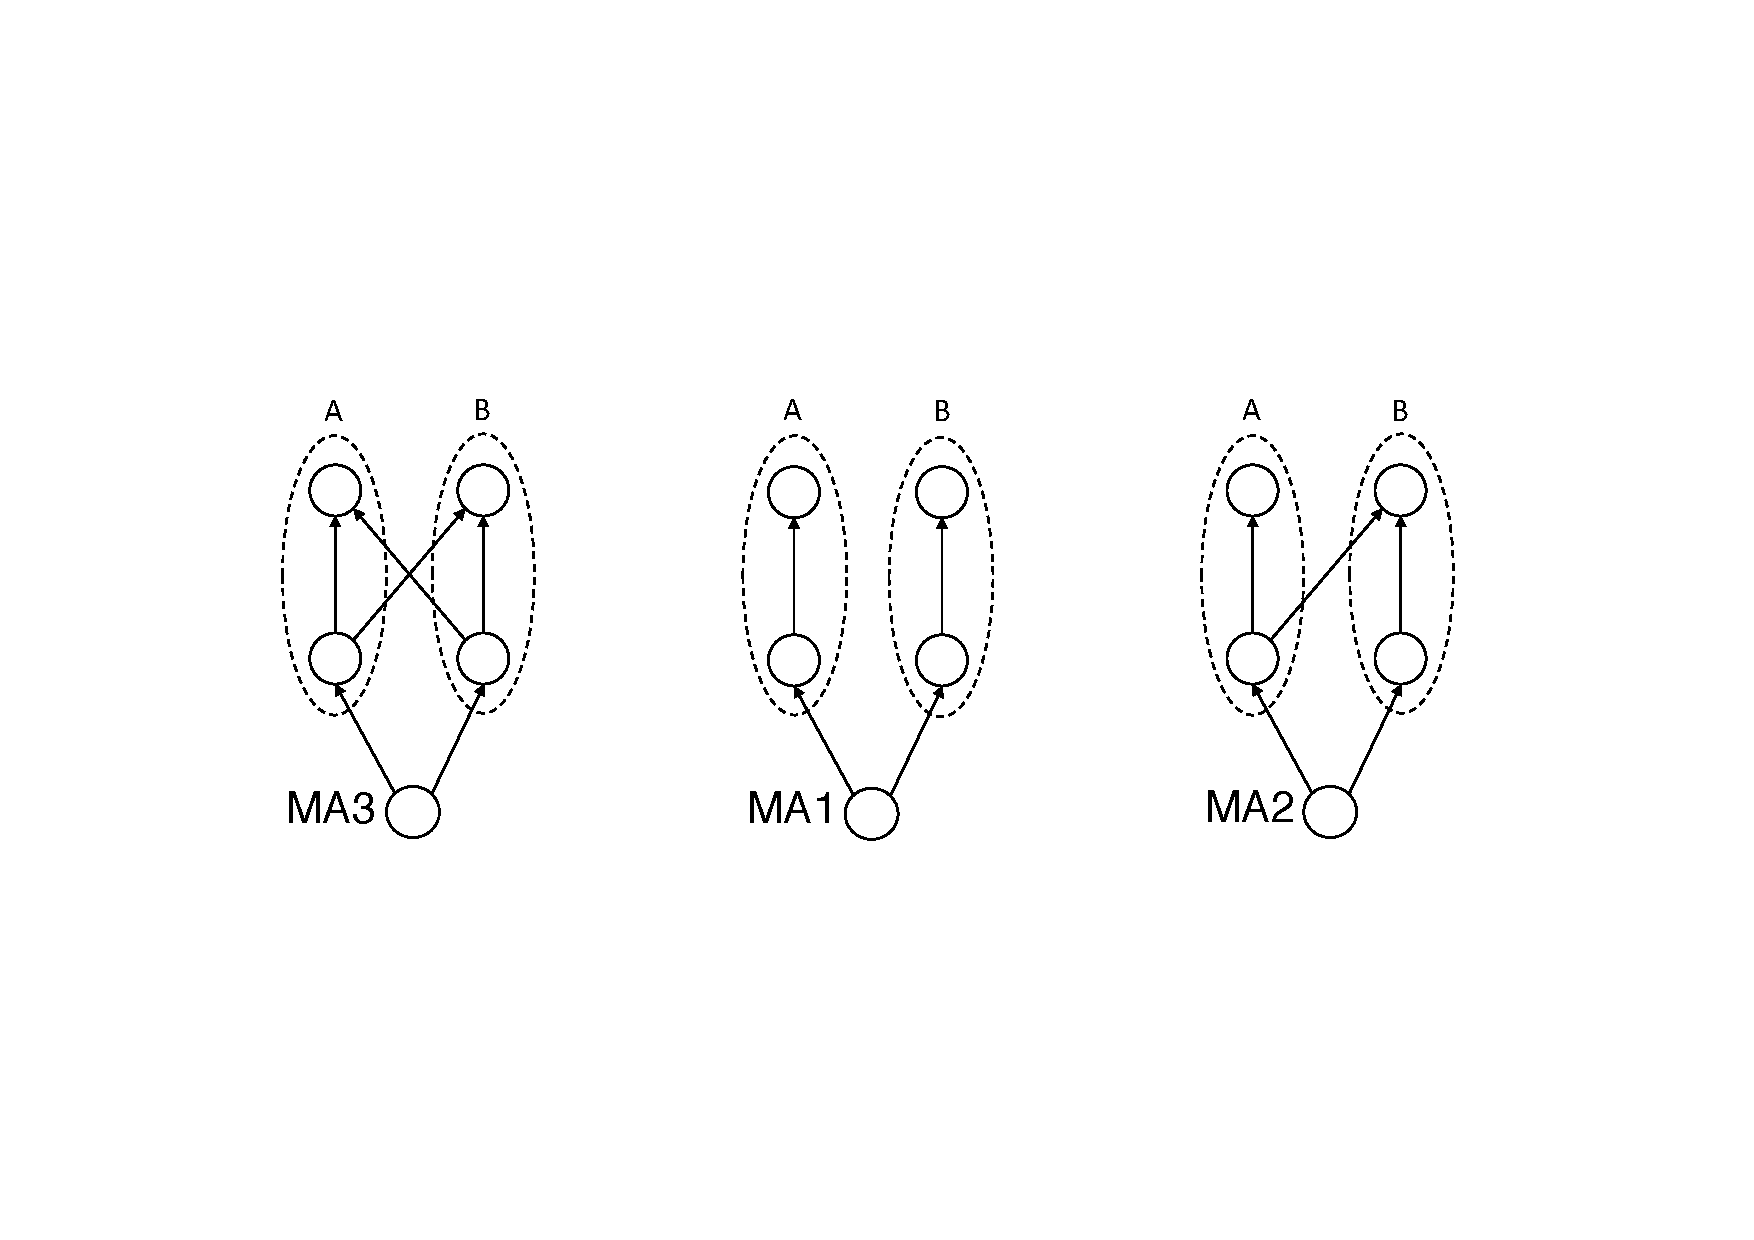
\includegraphics[width=\linewidth]{figs/mutualpositions}
\caption{Mutual arrangement of subgraphs $A$ and $B$}\label{fig:mutpos}
\end{figure}

\begin{definition}
\label{def:mutpos}
The mutual arrangement of two subgraphs $A$ and $B$ may be (Figure \ref{fig:mutpos}):
\begin{itemize}
\item \textbf{MA1:} $A$ and $B$ are independent, if there does not exist a pair of vertices of the two subgraphs, for which one vertex depends on another.
\item \textbf{MA2:} Uni-dependent ($A$ depends on $B$), if there exists a vertex $v$ in $B$ and $A$ depends on $v$, but there does not exist a vertex in $A$ on which $B$ depends.
\item \textbf{MA3:} Cross-dependent ($A$ and $B$ are cross-dependent if there exist vertices $v$ in $A$, $u$ in $B$ and $B$ depends on $v$, $A$ depends on $u$.
\end{itemize}
\end{definition}

\begin{figure}[h]
\centering
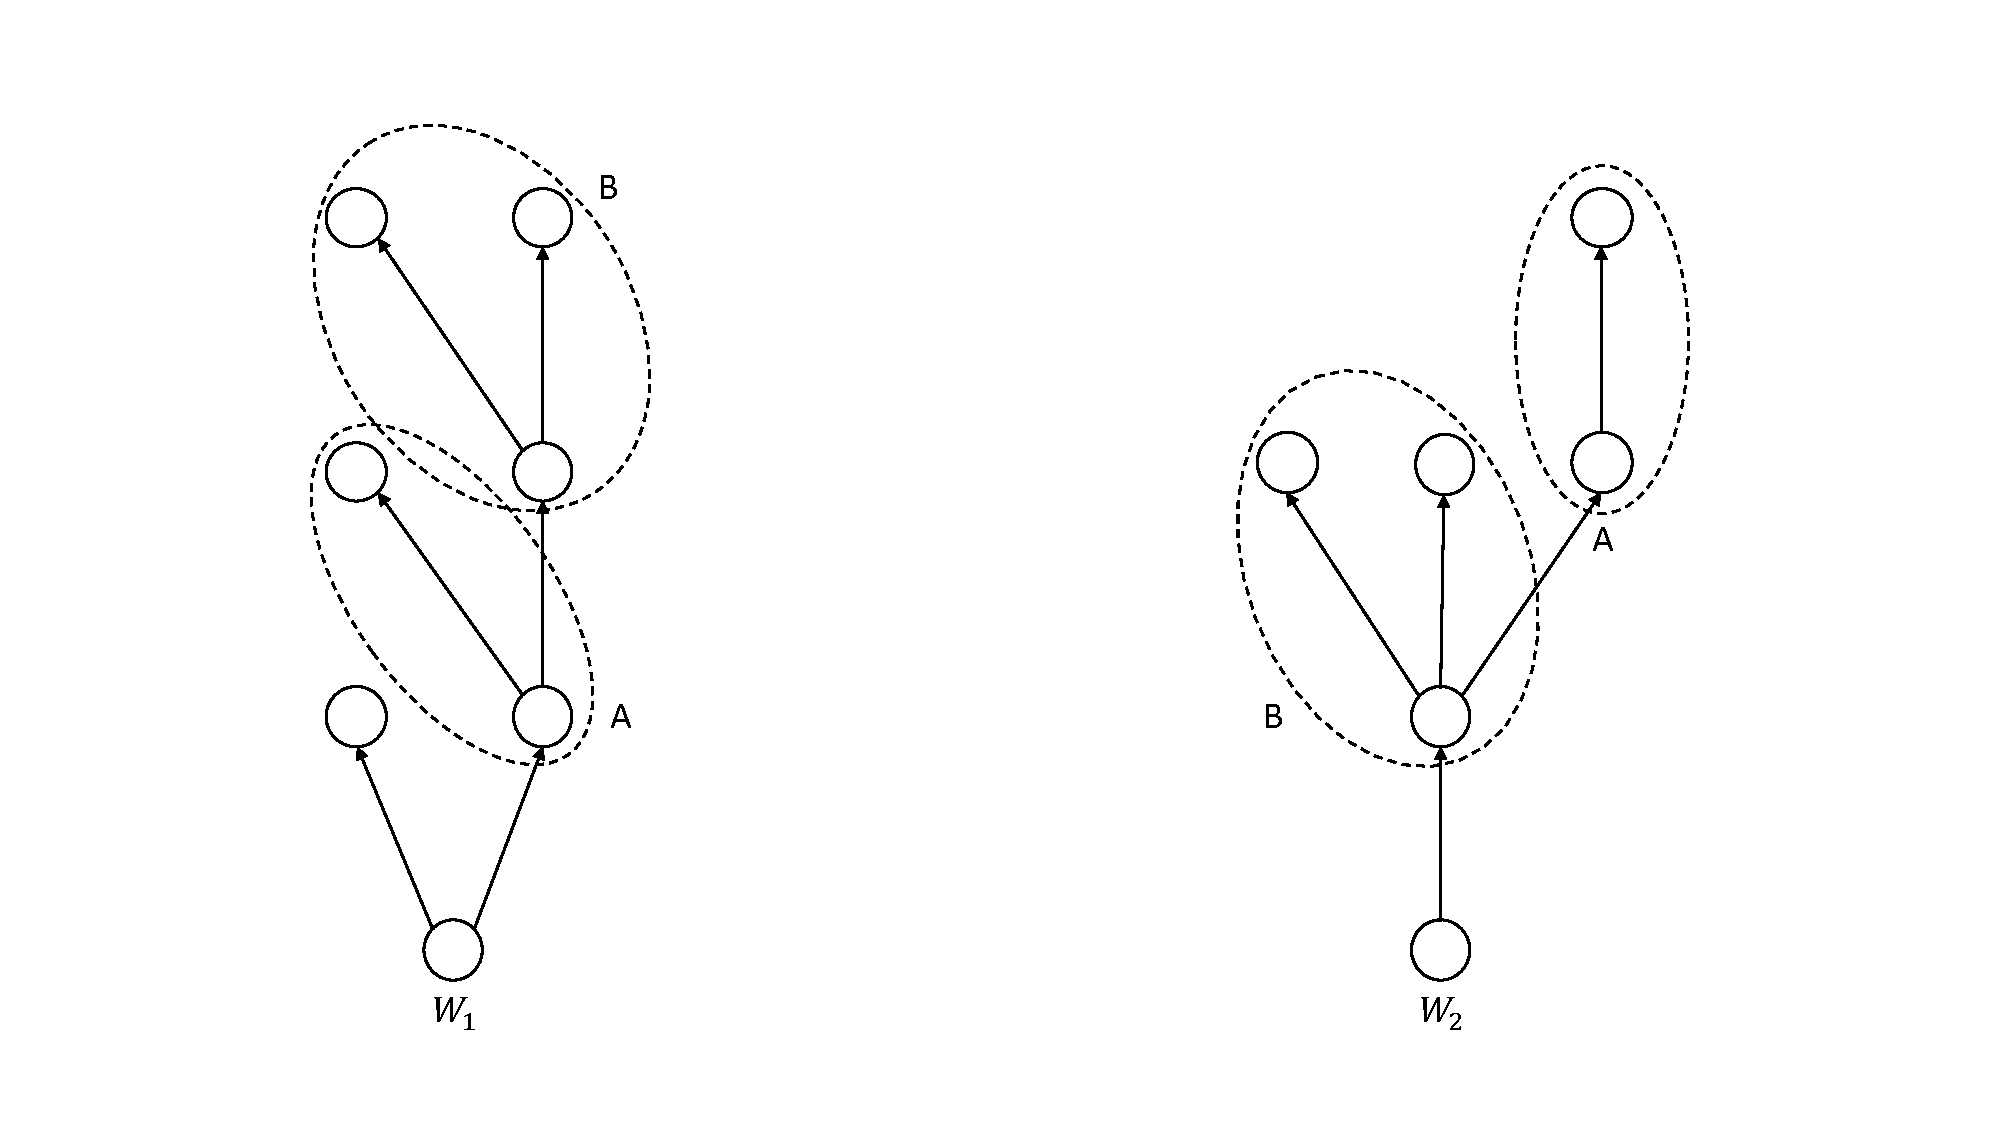
\includegraphics[width=\linewidth]{figs/cross-dep_of_2_w}
\caption{Cross-dependency of common-parts $A$ and $B$ in workflows $W_1$ and $W_2$}\label{fig:cross-dep_of_2_w}
\end{figure}


Depending on the mutual arrangement of subgraphs that belong to common parts of workflows (within or across workflows), it may or not be possible to perform joint execution of more than one common parts. We will showcase this with an example. Let us consider the two workflows $W_1$ and $W_2$ that have two common parts, $A$ and $B$. Joint execution of both $A$ and $B$ is not possible if:
\begin{itemize}
\item At least in one workflow the subgraphs of common parts $A$ and $B$ are cross-dependent (MA3).
\item In workflow $W_1$ common part $A$ depends on common part $B$ (MA2) and in $W_2$ $B$ depends on $A$ (MA2), as depicted in Figure \ref{fig:cross-dep_of_2_w}.
\end{itemize}

We will devise techniques in order to discover efficient dependencies of common parts. Towards this goal we will be inspired by the problem and solutions of the Longest and Heaviest Increasing Subsequence \cite{Jacobson:1992:HIS:647812.738135,Yang:2005:FAC:1710865.1711092}, which seem very promising for dealing with such situations.



\chapter{Related Work}\label{chapt:related}
Most Workflow Management Systems (WMS) are described in the report D5.1~\cite{d5.1}. In this chapter we discuss only works that engage in optimization.

Workflow management systems have emerged in order to provide easy-to-use specification of tasks that have to be performed during data analysis. An essential problem that these systems need to solve is the combination of various tools for workflow execution and optimization over multiple engines into a single research analysis / system. The field of workflow management is a relatively new field of research, but there are already some promising results.

The HFMS system~\cite{6544907} builds on top of previous work on multi-engine execution optimization~\cite{Simitsis:2012:OAD:2213836.2213963}. This research focuses on optimization and execution across multiple engines.
The design of flows in HFMS is agnostic to a physical implementation. Data sets need not be bound to a data store, and operators need not be bound to an execution engine. HFMS handles flows as DAGs encoded in xLM, a proprietary language for expressing data flows.

Work related to HFMS~\cite{5447816} and~\cite{Simitsis:2012:OAD:2213836.2213963} focuses on optimizing flows for several objectives: performance, fault-tolerance and freshness over multiple execution engines.
Optimization is defined as a search space problem. These states are obtained by a large number of possible transitions: swap, factorize, distribute, compose, decompose, partition, add recovery point, replicate, parallelization, function shipping, data shipping, etc. Due the vastness of the state space, some techniques / heuristics are proposed to prune it.
To assess the cost of states functions are defined both for operations (each vertex in a flow graph) and transitions. The work in~\cite{Simitsis:2013:XPA:2463676.2465247} describes the process of construction of cost functions in more detail, and shows how they can be defined by engineer or during test runs or using micro-benchmarks.
The experiments demonstrate the feasibility of their technique by comparing the heuristic solutions to those found by exhaustive search.

Thus, a significant difference of the HFMS system and related works from our research is that we are tackling and aim to propose solutions for a wider statement of the problem:  the development of WMT in  ASAP  aims to manage workflows that have a variety of heterogeneous formats and can be processed on a variety of heterogeneous engines that may be, furthermore, distributed. Beyond this, the main difference of our research with HFMS and related works is that the latter focuses only on single-workflow optimization, whereas  the first will focus also on multi-workflow optimization. %Nevertheless, their approach to optimization is extremely relevant to the objectives of ASAP and we believe that we can leverage this knowledge and generalize it in a more all-around framework.

\chapter{Summary}\label{chapt:summary}
This document describes the first version of WMT. This includes the declaration semantics of the workflow, design, analysis and optimization modules. Furthermore, we depict the work of WMT on specific use cases from the telecommunication and web analytics domains.Finally, we make an initial discussion on multi-workflow optimization. 

\bibliographystyle{plain}
\bibliography{biblio}

\end{document}